%
% Copyright � 2015 Peeter Joot, Xingqi Zhang.  All Rights Reserved.
%
\documentclass[handout]{beamer}
\setbeamertemplate{navigation symbols}{}

\usetheme{Warsaw}
%\usepackage{ngerman}
\beamersetuncovermixins{\opaqueness<1>{25}}{\opaqueness<2->{15}}

\PassOptionsToPackage{square,numbers}{natbib}

\usepackage{figpath}

% args: scale, filename
\newcommand{\onefigure}[2]{%
\includegraphics[#1]{\figpath{}#2}%
}

% args: scale, filename, caption
%\newcommand{\makefigure}[3]{%
%\begin{figure}%
%\onefigure{scale=#1}{#2}\caption{#3}%
%\end{figure}%
%}
\newcommand{\makefigure}[3]{%
\begin{figure}%
\onefigure{scale=#1}{#2}%
\end{figure}%
}

% doesn't work with these other packages.
%\usepackage{floatrow}%
% args: (scale, filename, caption) x 2
%\newcommand{\twofigures}[6]{%
%\begin{figure}[!h]%
%	\begin{floatrow}%
%		\includegraphics[scale=#1]{\figpath{}#2}\caption{#3}%
%		\includegraphics[scale=#4]{\figpath{}#5}\caption{#6}%
%	\end{floatrow}%
%\end{figure}%
%}

\usepackage{subfig}

% scale, path, scale, path, caption
%\newcommand{\twofigures}[5]{%
%\begin{figure}%
%\centering%
%\subfloat[][]{\onefigure{scale=#1}{#2}}%
%\qquad%
%\subfloat[][]{\onefigure{scale=#3}{#4}}%
%\caption{#5}%
%\end{figure}%
%}
\newcommand{\twofigures}[5]{%
\begin{figure}%
\centering%
\subfloat[][]{\onefigure{scale=#1}{#2}}%
\qquad%
\subfloat[][]{\onefigure{scale=#3}{#4}}%
\end{figure}%
}

\usepackage{natbib}
\usepackage{siunitx}
\usepackage{scrfontsizes}
\usepackage{tikz}

%(1) Title with your name (1 page)
%(2) Introduction (1 page)
%(3) Description of the topic/problem (1 page)
%(4) Historical overview of the topic (1 page)
%(5) Reflectarray Design Overview (1 page)
%(6) Theory/Analysis (5 page)
%(7) Advantages/Disadvantages (1 page)
%(8) Bandwidth Considerations (1 page)
%    Bandwidth Enhancement Methods
%(9) Application(s) (4-5 page)
%    Reconfigurable/scannable reflectarrays
%(10) Transmitarray (1 page)
%(11) Future directions (2-1 page)
%(12) Summary (1 page)
%(13) Bibliography (at least 10 references) (1 page)

\begin{document}
\title{Reflectarray}
\author{Xingqi Zhang, Haroon Siddiqui, Peeter Joot}

\date{\today}

\begin{frame}
\titlepage
\end{frame}

\begin{frame}
\frametitle{Table of contents}
\tableofcontents
\end{frame}


%------------------------------------------------
\section{Overview}

\begin{frame}
\frametitle{Introduction}
	\text{Long distance communications: high-gain antennas}
	\vspace*{-3mm}
	\begin{center}
	\hspace*{-10mm}
	  \begin{tikzpicture}
			\node at(-2,2.5){Parabolic Reflector}; %www.naturaecoenergy.com
			\node at(-1.6,0.5){\includegraphics[scale=0.177,clip,trim={2cm 0cm 2cm 0cm}]{../../figures/ece1229/project/Parabolic.jpg}};
			\node at(2,2.5){Phased Arrays}; %www.activefrance.com
			\node at(1.6,0.5){\includegraphics[scale=0.5,clip,trim={0cm 0.7cm 0cm 0cm}]{../../figures/ece1229/project/Phased_array.jpg}};

				\node at(-4.8,0.5){\begin{minipage}{3cm}
						\small 
						\begin{itemize}%\setlength\itemsep{1.2em}
								\item Simple and well developed%\\[0.5em]
								\item Bulky, hard to manufacture
								\item Limited beam scanning
							   \end{itemize}
					\end{minipage}};

				\node at(4.6,0.5){\begin{minipage}{3cm}
						\small 
						\begin{itemize}%\setlength\itemsep{1.2em}
								\item Flexible beams and low profile%\\[0.5em]
								\item Expensive
								\item Power inefficiency
							   \end{itemize}
					\end{minipage}};
	\vspace*{2mm}
										
			 \draw[->,double=white](-1.8,-0.9)to[out=0,in=115,looseness=0.9](-1,-1.45);
				\draw[->,double=white](1.8,-0.9)to[out=180,in=180-115,looseness=0.9](1,-1.45);

			\node at(0,-1.82){Reflectarray Antenna ("Flat Reflector")}; %www.activefrance.com

				\node at(0,-2.6){\begin{minipage}{10cm}
						\small 
						\begin{itemize}%\setlength\itemsep{1.2em}
								\item Mitigate the disadvantages and combine certain advantages of reflector antennas and phased arrays
								%\item 
							   \end{itemize}
					\end{minipage}};

		\end{tikzpicture}
		
\end{center}				



\end{frame}

%------------------------------------------------
\begin{frame}
\frametitle{Historical overview}

	\begin{center}
	\hspace*{-15mm}
	  \begin{tikzpicture}
			\node at(-4,0){\includegraphics[scale=0.4,clip,trim={0cm 0cm 0cm 0cm}]{../../figures/ece1229/project/history1.png}};
			\node at(0,0){\includegraphics[scale=0.4,clip,trim={0cm 0cm 0cm 0cm}]{../../figures/ece1229/project/history2.png}};
			\node at(4,0){\includegraphics[scale=0.45,clip,trim={0cm 0cm 0cm 0cm}]{../../figures/ece1229/project/history3.png}};

				\node at(-4.3,3){\begin{minipage}{5cm}
						\begin{itemize}%\setlength\itemsep{1.2em}
								\item Waveguide Reflectarray (Kennedy, 1960s) \citep{Berry1963}\\[1em]
							   \end{itemize}
					\end{minipage}};

				\node at(0,3){\begin{minipage}{5cm}
						\begin{itemize}%\setlength\itemsep{1.2em}
								\item Spiralphase Reflectarray  (Phelan, 1970s) \citep{Phelan1977}\\[1em]
							   \end{itemize}
					\end{minipage}};
				
				\node at(4.3,3){\begin{minipage}{5cm}
						\begin{itemize}%\setlength\itemsep{1.2em}
								\item Microstrip Reflectarray (Malagisi, 1980s) \citep{Malagisi1978}\\[1em]
							   \end{itemize}
					\end{minipage}};	
									
		\end{tikzpicture}
		
\end{center}	

\end{frame}

%------------------------------------------------
\section{Analysis/Design}

\begin{frame}
\frametitle{Reflectarray Antenna}

	\begin{center}

	\vspace*{-0.6cm}
	\hspace*{-5mm}
	  \begin{tikzpicture}
			\node at(0,0){\includegraphics[scale=0.5,clip,trim={0cm 0cm 0cm 0cm}]{../../figures/ece1229/project/description.png}};


				\node at(0,-3.5){\begin{minipage}{11.5cm}
						\begin{itemize}%\setlength\itemsep{1.2em}
								\item \small An antenna consisting of either a flat or a slightly curved reflecting surface and an illuminating feed antenna;
								\item \small The feed antenna spatially illuminates the radiating elements on the reflecting surface;
								\item \small These radiating elements are predesigned to reradiate and scatter the incident field with electrical phases;
								\item \small A planar phase front is formed in the far-field distance.
						
						\end{itemize}
					\end{minipage}};
									
		\end{tikzpicture}
\end{center}	

\end{frame}
		
%------------------------------------------------
\begin{frame}
\frametitle{Reflectarray Elements}
	\hspace*{-3mm}
	\text{Several methods for reflectarray elements to achieve a planar phase front.}

	\begin{center}

	%\vspace*{-0.6cm}
	\hspace*{-10mm}
	  \begin{tikzpicture}
			\node at(2.4,0){\includegraphics[scale=0.6,clip,trim={0cm 0cm 0cm 0cm}]{../../figures/ece1229/project/elements.png}};

				\node at(-4,0){\begin{minipage}{7.75cm}
						\begin{itemize}%\setlength\itemsep{1.2em}
								\item \small Identical microstrip patches with variable-length phase delay lines: compensate for the phase delays over the different paths from the illuminating feed;\\[0.5em]
								\item \small Variable-size patches, dipoles, or rings: different scattering impedances and, thus, different phases to compensate for the different feed-path delays;\\[0.5em]
								\item \small  All identical circularly polarized elements but with different angular rotations: compensate for the feed path–length differences (circular polarization only).
						
						\end{itemize}
					\end{minipage}};
									
		\end{tikzpicture}
\end{center}	

\end{frame}
%------------------------------------------------
\begin{frame}
\frametitle{Reflectarray Analysis}
	\hspace*{-3mm}
	%\text{The operating principle can be explained by considering the reflectarray in transmitting mode with a horn antenna located in a centered or offset position, and assuming that the reflectarray elements are in the far-field region of the horn.}
	\begin{center}
	\vspace*{-5mm}
	\hspace*{-10mm}
	  \begin{tikzpicture}
			\node at(2.5,0){\includegraphics[scale=0.6,clip,trim={0cm 0cm 0cm 0cm}]{../../figures/ece1229/project/analysis.png}};

				\node at(-4,0){\begin{minipage}{7.55cm}
						\begin{itemize}%\setlength\itemsep{1.2em}
								\item \small The operating principle: Considering the reflectarray in transmitting mode with a horn antenna located in a centered or offset position, and assuming that the reflectarray elements are in the far-field region of the horn.
								\item \small Incident wave: Locally considered as a plane wave with a phase proportional to the distance from the phase center of the feed-horn to each element;
								\item \small Progressive phase distribution: Convert the spherical wave into a focused beam.
						
						\end{itemize}
					\end{minipage}};
									
		\end{tikzpicture}
\end{center}	

\end{frame}

%------------------------------------------------
\begin{frame}
\frametitle{Phase-Shift Distribution}
	%\text{The phase-shift that must be introduced at each element to produce a collimated beam in a given direction is determined in this section.}

	\begin{center}
	%\vspace*{-0.6cm}
	\hspace*{-10mm}
	  \begin{tikzpicture}
			\node at(2.5,0){\includegraphics[scale=0.6,clip,trim={0cm 0cm 0cm 0cm}]{../../figures/ece1229/project/phase.png}};

				\node at(-4,2.2){\begin{minipage}{7cm}
						\begin{itemize}%\setlength\itemsep{1.2em}
								\item \small Progressive phase distribution on the reflectarray surface produceing a beam in the direction $(\theta_b,\varphi_b)$: $\phi(x_i,y_i)=-k_0\sin{\theta_b}\cos{\varphi_b}x_i-k_0\sin{\theta_b}\sin{\varphi_b}y_i$;
						\end{itemize}
					\end{minipage}};
				
				\node at(-4,0){\begin{minipage}{7cm}
						\begin{itemize}%\setlength\itemsep{1.2em}
								\item \small Phase of the reflected field at each reflectarray element is equal to the phase of the incident field:\\[0.5em]
					$\phi(x_i,y_i)=-k_0d_i-\phi_R(x_i,y_i)$
						\end{itemize}
					\end{minipage}};									

				\node at(-4,-2){\begin{minipage}{7cm}
						\begin{itemize}%\setlength\itemsep{1.2em}
								\item \small The phase-shift required at each element: $\phi_R=k_0(d_i-(x_i\cos{\varphi_b}+y_i\sin{\varphi_b})\sin{\theta_b})$
						
						\end{itemize}
					\end{minipage}};		


		\end{tikzpicture}
\end{center}	
\end{frame}

%------------------------------------------------
\begin{frame}
\frametitle{Reflectarray Design}
	\begin{center}
	%\vspace*{-5mm}
	\hspace*{-10mm}
	  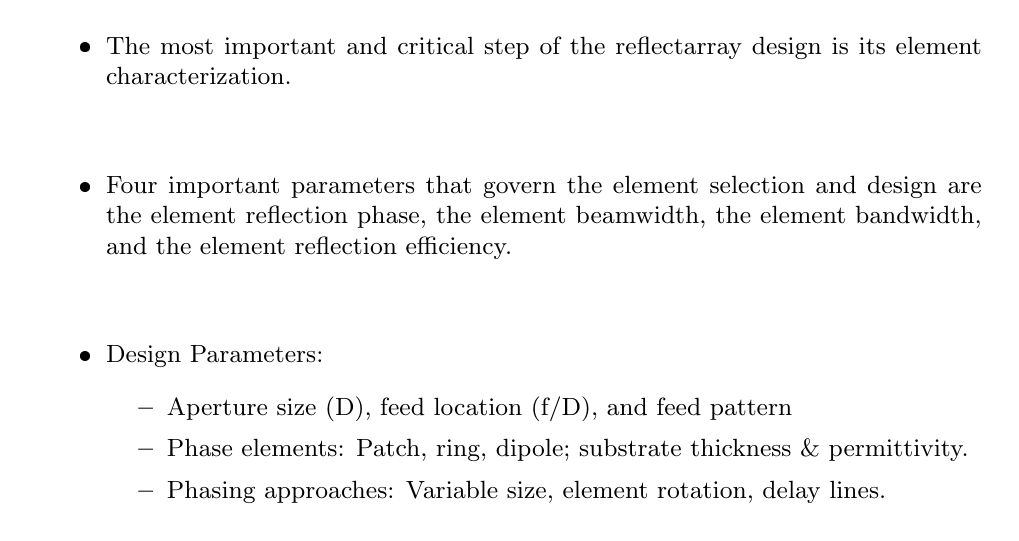
\begin{tikzpicture}
			%\node at(2.5,0){\includegraphics[scale=0.6,clip,trim={0cm 0cm 0cm 0cm}]{../../figures/ece1229/project/analysis.png}};

				\node at(0,0){\begin{minipage}{12cm}
						\begin{itemize}%\setlength\itemsep{1.2em}
								\item \small The most important and critical step of the reflectarray design is its element characterization.\\[1em]
								\item \small  Four important parameters that govern the element selection and design are the element reflection phase, the element beamwidth, the element bandwidth, and the element reflection efficiency. \\[1em]
								\item \small  Design Parameters:
												\begin{itemize}%\setlength\itemsep{1.2em}
								             \item \small Aperture size (D), feed location (f/D), and feed pattern
								             \item \small Phase elements: Patch, ring, dipole; substrate thickness \& permittivity.
								             \item \small Phasing approaches: Variable size, element rotation, delay lines.
												\end{itemize}

						\end{itemize}
					\end{minipage}};
									
		\end{tikzpicture}
\end{center}	

\end{frame}


%------------------------------------------------
\begin{frame}
%\frametitle{Element Effects and Selection}
\frametitle{Reflectarray Design Tools}

	\begin{center}
	\hspace*{-15mm}
	  \begin{tikzpicture}
			\node at(-4,0){\includegraphics[scale=0.4,clip,trim={0cm 0cm 0cm 0cm}]{../../figures/ece1229/project/tool1.png}};
			\node at(0,0){\includegraphics[scale=0.35,clip,trim={0cm 0cm 0cm 0cm}]{../../figures/ece1229/project/tool2.png}};
			\node at(4,0){\includegraphics[scale=0.4,clip,trim={0cm 0cm 0cm 0cm}]{../../figures/ece1229/project/tool3.png}};

			\node at(-4.3,4.5){Analysis Tools};
			\node at(0,4.5){Optimization Tools};
			\node at(4.3,4.5){Measurement Tools};


				\node at(-4.3,3){\begin{minipage}{4.5cm}
						\begin{itemize}%\setlength\itemsep{1.2em}
								\item \small Radiation Analysis\\[0.5em]
									\item \small Efficiency Analysis\\[0.5em]
								\item \small Phase Error Analysis
						   \end{itemize}
					\end{minipage}};

				\node at(0,3){\begin{minipage}{4.5cm}
						\begin{itemize}%\setlength\itemsep{1.2em}
								\item \small Alternating Projection Method (APM)\\[0.5em]
								\item \small Particle Swarm Optimization (PSO)
							   \end{itemize}
					\end{minipage}};
				
				\node at(4.3,3){\begin{minipage}{4.5cm}
						\begin{itemize}%\setlength\itemsep{1.2em}
								\item \small Spectral Near-to-Far-Field (NTFF) Transformation\\[0.5em]
								\item \small Microwave Holography
							   \end{itemize}
					\end{minipage}};	
									
		\end{tikzpicture}
		
\end{center}

\end{frame}



%------------------------------------------------


\section{Discussion}
%(1 page)
\begin{frame}
\frametitle{Advantages}

\begin{itemize}
\item Flat.
\item Low losses.
\item No need to feed the patch elements directly.
\item Phase shifting electronics for each patch element is not required, lowering cost.
\item Reconfiguration and scanning is possible if phase shifting electronics are included.
\item Large aperture reflectarrays can be folded more easily than parabolic equivalents (for space applications).
\item Like parabolic reflectors, multiple beam capability is possible with additional feed sources.
\item Variable sized patch elements can lead to low cross-polarization.
\end{itemize}
\end{frame}

\begin{frame}
\frametitle{Disadvantages}

\begin{itemize}
\item Narrow bandwidth, due to narrow bandwidth of patch elements (3-5\%)
\item Differential spatial phase delays limit bandwidth, due to sensitivity of phase to the resonance frequencies.
\citep{pozar1997design}
%FIXME: Huang discusses this latter point as a major source of limited bandwidth,
%but doesn't make it clear why there is a connection between the phase differences at points in the array
%and how that relates to the overall bandwidth limitation.
\item Bandwidth limited by physical extent of the array, limiting space applications.
\citep{encinar2001design}
\end{itemize}
\end{frame}

%\begin{frame}[allowframebreaks]
\begin{frame}
\frametitle{Bandwidth Improvement}
\begin{itemize}
\item Stacked layers can reduce phase range limitations (to several times \ang{360}).
\citep{pozar1997design}
\item Delay lines aperture-coupled to printed patches.  Used to achieve 20 \% bandwidth in 80 \si{cm} reflectarray.
\citep{encinar2010recent}
\item Multifacet (\( 2 \si{m} \times 0.5 \si{m} \)) designs can reduce spatial phase delays.  
%Both very large fixed piecewise flat configurations, as well as some very clever unfolding to parabolic designs .
%\makefigure{0.15}{huangFig58multifacet.png}{Multifacet reflectarray}
%huang7_58BpiecewiseFlatParabolic.png
%huang7_58ApiecewiseFlatParabolic.png
\makefigure{0.15}{huang7_58BpiecewiseFlatParabolic.png}{Multifacet \( 2 \si{m} \times 0.5 \si{m} \) reflectarray}
\end{itemize}
\end{frame}


\begin{frame}
\frametitle{Applications: Solar cell hybrid reflectarray.}

\begin{itemize}
\item Can be combined with solar cells to provide both power and antenna function. %\cref{fig:huang:huangFig2_10_solarCellWithRA}.
Small crossed dipole patches do not significantly inhibit solar cell performance. \citep{huang2008reflectarray}
\makefigure{0.15}{huangFig2_10_solarCellWithRA.png}{Hybrid solar cell reflectarray \citep{huang2008reflectarray}}
\end{itemize}
\end{frame}

\begin{frame}
\frametitle{Applications: Inflatable reflectarray.}

\begin{itemize}
\item
Example of 1 \si{m} 8.3 \si{GHz} (X-band), and 3 \si{m} 32 \si{GHz} (Ka-band) reflectarrays.  The 3\si{m} array has 200000 elements!
\end{itemize}

\twofigures{0.2}{huang7_1_inflatable1meter.png}{0.27}{huang7_3_inflatable3m.png}{1 \si{m} X-band and 3 \si{m} Ka-band inflatable reflectarrays (JPL and ILC Dover).}
\end{frame}

\begin{frame}
\frametitle{Applications: Contoured beam applications.}

\begin{itemize}
\item It can be desirable to have a beam that targets multiple geographies.
\item Don't want to waste power on unpopulated areas.
\item Example: 12 \si{GHz}, 1 \si{m} three-layer reflectarray for geostationary targeting of three regions. From: \citep{encinar2004three}
\end{itemize}

\makefigure{0.3}{threeLayerReflectarrayContouredBeamEncinarPaperFig3.png}{Geostationary targeting of three regions. From: \citep{encinar2004three}}
\end{frame}

%TODO: 4-5 page.  2 left.

\begin{frame}
\frametitle{Transmitarray (array lenses)}
\begin{itemize}
\item Feed from behind the array instead of centered or offset reflected feed.  From: \citep{lau2012reconfigurable}
\makefigure{0.15}{lau_jonathan_figure1_2_transmitarray.png}{transmitarray feed configuration.  From: \citep{lau2012reconfigurable}}
\item Can avoid blocking the beam with the feed.
\item Design care is required to avoid undesirable reflection off the back surface.
\item With less reliance on ground plane reflection and resonance than reflectarrays, higher bandwidth designs may be possible.
\end{itemize}
\end{frame}

\begin{frame}[allowframebreaks]
\frametitle{Future directions}
\begin{itemize}
\item Gathered elements with common phase control has been used/proposed to reduce the number of active control devices for scannable and reconfigurable devices.  \citep{carrasco2012recent}
\item Multi-beam configurations with a single feed. \citep{carrasco2012recent}
\item Sub-reflectarrays in parabolic configuration for beam scanning.  \citep{arrebola2010phase} describes \( \pm \ang{12} \) scanning for 12 \si{GHz} 1 meter parabolic dish with 22 \si{cm} reflectarrays.
\item LCD substrates.  Bias voltages can alter the dielectric constant of the substrate.  Sub-millimeter (\si{Thz}) scanning reflectarrays have been demonstrated using this method.
\item ``Folded'' reflectarray.  The feed is put inline or behind the patch elements, with a polarizing grid above the array elements.
\twofigures{0.2}{huang_foldedSchematicFig7_45a.png}{0.27}{huang_foldedRenderingFig7_45b.png}{Folded reflectarray.}
\end{itemize}
\end{frame}

%TODO: 2-1 page

\begin{frame}
\frametitle{Summary}

\begin{itemize}
\item Desirable physical characteristics (flat, foldable, ...)
\item Can be manufactured with printed circuit techniques (relatively cheap, once designed).
\item Large variety of applications (space, ground, ...)
\item Can be combined with other techniques (arrays of reflectarrays, electronic phase control, ...)
\item Satisfactory solutions to original bandwidth limitations have been devised.
\item Active research area.
\end{itemize}

\end{frame}


\begin{frame}[plain]
%\begin{frame}[allowframebreaks,plain]
\frametitle{Bibliography}
\changefontsizes{7}
\bibliography{Bibliography}
\bibliographystyle{plainnat}
\end{frame}

\end{document}
